\documentclass[twoside]{book}

% Packages required by doxygen
\usepackage{calc}
\usepackage{doxygen}
\usepackage{graphicx}
\usepackage[utf8]{inputenc}
\usepackage{makeidx}
\usepackage{multicol}
\usepackage{multirow}
\usepackage{fixltx2e}
\PassOptionsToPackage{warn}{textcomp}
\usepackage{textcomp}
\usepackage[nointegrals]{wasysym}
\usepackage[table]{xcolor}

% Font selection
\usepackage[T1]{fontenc}
\usepackage{mathptmx}
\usepackage[scaled=.90]{helvet}
\usepackage{courier}
\usepackage{amssymb}
\usepackage{sectsty}
\renewcommand{\familydefault}{\sfdefault}
\allsectionsfont{%
  \fontseries{bc}\selectfont%
  \color{darkgray}%
}
\renewcommand{\DoxyLabelFont}{%
  \fontseries{bc}\selectfont%
  \color{darkgray}%
}
\newcommand{\+}{\discretionary{\mbox{\scriptsize$\hookleftarrow$}}{}{}}

% Page & text layout
\usepackage{geometry}
\geometry{%
  a4paper,%
  top=2.5cm,%
  bottom=2.5cm,%
  left=2.5cm,%
  right=2.5cm%
}
\tolerance=750
\hfuzz=15pt
\hbadness=750
\setlength{\emergencystretch}{15pt}
\setlength{\parindent}{0cm}
\setlength{\parskip}{0.2cm}
\makeatletter
\renewcommand{\paragraph}{%
  \@startsection{paragraph}{4}{0ex}{-1.0ex}{1.0ex}{%
    \normalfont\normalsize\bfseries\SS@parafont%
  }%
}
\renewcommand{\subparagraph}{%
  \@startsection{subparagraph}{5}{0ex}{-1.0ex}{1.0ex}{%
    \normalfont\normalsize\bfseries\SS@subparafont%
  }%
}
\makeatother

% Headers & footers
\usepackage{fancyhdr}
\pagestyle{fancyplain}
\fancyhead[LE]{\fancyplain{}{\bfseries\thepage}}
\fancyhead[CE]{\fancyplain{}{}}
\fancyhead[RE]{\fancyplain{}{\bfseries\leftmark}}
\fancyhead[LO]{\fancyplain{}{\bfseries\rightmark}}
\fancyhead[CO]{\fancyplain{}{}}
\fancyhead[RO]{\fancyplain{}{\bfseries\thepage}}
\fancyfoot[LE]{\fancyplain{}{}}
\fancyfoot[CE]{\fancyplain{}{}}
\fancyfoot[RE]{\fancyplain{}{\bfseries\scriptsize Generated on Sun Apr 27 2014 20\+:03\+:03 for My Project by Doxygen }}
\fancyfoot[LO]{\fancyplain{}{\bfseries\scriptsize Generated on Sun Apr 27 2014 20\+:03\+:03 for My Project by Doxygen }}
\fancyfoot[CO]{\fancyplain{}{}}
\fancyfoot[RO]{\fancyplain{}{}}
\renewcommand{\footrulewidth}{0.4pt}
\renewcommand{\chaptermark}[1]{%
  \markboth{#1}{}%
}
\renewcommand{\sectionmark}[1]{%
  \markright{\thesection\ #1}%
}

% Indices & bibliography
\usepackage{natbib}
\usepackage[titles]{tocloft}
\setcounter{tocdepth}{3}
\setcounter{secnumdepth}{5}
\makeindex

% Hyperlinks (required, but should be loaded last)
\usepackage{ifpdf}
\ifpdf
  \usepackage[pdftex,pagebackref=true]{hyperref}
\else
  \usepackage[ps2pdf,pagebackref=true]{hyperref}
\fi
\hypersetup{%
  colorlinks=true,%
  linkcolor=blue,%
  citecolor=blue,%
  unicode%
}

% Custom commands
\newcommand{\clearemptydoublepage}{%
  \newpage{\pagestyle{empty}\cleardoublepage}%
}


%===== C O N T E N T S =====

\begin{document}

% Titlepage & ToC
\hypersetup{pageanchor=false,
             bookmarks=true,
             bookmarksnumbered=true,
             pdfencoding=unicode
            }
\pagenumbering{roman}
\begin{titlepage}
\vspace*{7cm}
\begin{center}%
{\Large My Project }\\
\vspace*{1cm}
{\large Generated by Doxygen 1.8.7}\\
\vspace*{0.5cm}
{\small Sun Apr 27 2014 20:03:03}\\
\end{center}
\end{titlepage}
\clearemptydoublepage
\tableofcontents
\clearemptydoublepage
\pagenumbering{arabic}
\hypersetup{pageanchor=true}

%--- Begin generated contents ---
\chapter{D\+G\+R Framework (D\+I\+S\+T\+R\+I\+B\+U\+T\+E\+D G\+R\+A\+P\+H\+I\+C\+S R\+E\+N\+D\+E\+R\+E\+R) (pronounced \char`\"{}\+Dogger\char`\"{})}
\label{md_README}
\hypertarget{md_README}{}
Written by Brent Nix (bjnix at mtu dot edu) and James Walker (jwwalker at mtu dot edu), with some modifications by Scott A. Kuhl (kuhl at mtu dot edu)

\subsection*{O\+V\+E\+R\+V\+I\+E\+W }

Originaly meant for distributed graphics rendering, D\+G\+R is a small lightweight general use framework that allows for syncing data between servers with minimal code intrusion. It takes primitive data types by default, but can be configured to accept any data type, structure, or object.

\subsection*{H\+O\+W I\+T W\+O\+R\+K\+S }

Here is an overview of how D\+G\+R works\+:

The M\+A\+S\+T\+E\+R program forwards state data via U\+D\+P packets to the relay program running on the head node of the cluster.

The R\+E\+L\+A\+Y, running on the head node of the cluster, listens for packets from the master program and automatically forwards them to an I\+P address (which could be a broadcast address, and is by default).

The S\+L\+A\+V\+E\+S listen for packets on the appropriate port. Upon receipt, they immediately decode the packets and update their state with the data.

The basic premise here is a master -\/ slave relationship. The specifics of how this relationship is implemented is completely up to you, but examples are provided for some more common constructs. Here are the examples that we have implemented\+:

1) Having a master node that talks to a relay on a cluster head \begin{DoxyVerb}                                                           {slave}
                                                           {slave}
                                      {Master}--->{relay}--{slave}
                                                           {slave}
                                                           {slave}
\end{DoxyVerb}


2) Running directly off of the cluster head (the relay functionality is moved into the master code) \begin{DoxyVerb}                                                           {slave}
                                                           {slave}
                                         {master/relay}----{slave}
                                                           {slave}
                                                           {slave}
\end{DoxyVerb}


and finally, a purely local environment allows us to recreate the above situations for local testing purposes. \begin{DoxyVerb}                                                master
                                      {relay,slave,slave,slave,...}

                                                  or

                                             master/relay
                                      {slave,slave,slave,slave,...}
\end{DoxyVerb}


Some sample \char`\"{}run-\/scripts\char`\"{} have been included to help you get started\+:

Scripts specifically for Michigan Tech's I\+V\+S Display Wall\+:


\begin{DoxyItemize}
\item D\+G\+R\+Start\+I\+V\+S.\+sh
\item D\+G\+R\+Start\+I\+V\+S-\/startslaves.\+sh note\+: D\+G\+R\+Start\+I\+V\+S.\+sh calls D\+G\+R\+Start\+I\+V\+S-\/startslaves.\+sh
\end{DoxyItemize}

For testing on one machine\+:


\begin{DoxyItemize}
\item D\+G\+R\+Start\+Local.\+sh note\+: this may need some serious editing for your purposes
\end{DoxyItemize}

\subsection*{T\+O C\+O\+M\+P\+I\+L\+E T\+H\+E P\+A\+C\+K\+A\+G\+E\+S }


\begin{DoxyItemize}
\item Compile the package by typing \char`\"{}make\char`\"{}.
\item testing\+\_\+around.\+cpp has been provided as an example
\item This code should work with linux and O\+S\+X.
\item it has not been tested on windows and will likely not work without modification
\end{DoxyItemize}

\subsection*{D\+E\+V\+E\+L\+O\+P\+I\+N\+G Y\+O\+U\+R O\+W\+N D\+I\+S\+T\+R\+I\+B\+U\+T\+E\+D R\+E\+N\+D\+E\+R\+I\+N\+G P\+R\+O\+G\+R\+A\+M\+S }


\begin{DoxyItemize}
\item The testing\+\_\+around.\+cpp demo illustrates how to accomplish distributed rendering on a graphics cluster using only U\+D\+P packets, without relying on libraries such as Chromium.
\item D\+G\+R is independent of the windows composter or graphics libraries so it allows you to sync renderings between different windows managers and operating systems, having separate slave implementations for each.
\item Because D\+G\+R is a memory synchronizer, you can extend this concept for any distributed computation purposes, not just graphics.
\item You must include \char`\"{}\+D\+G\+R\+\_\+framework\char`\"{} in the files that you wish to use D\+G\+R in as well as compile your code with \char`\"{}\+D\+G\+R\+\_\+framework.\+cpp\char`\"{}
\item Because the source code for the master and slaves may be almost identical, you can have both binaries compiled out of the same source file. The code below demonstrates how to use preprocessor directives to separate out parts that are different between the master and the slave. I don't think that I have to mention that some care should be taken when choosing how to cut the code up. {\bfseries note\+:} {\itshape use -\/\+D\+D\+G\+R\+\_\+\+M\+A\+S\+T\+E\+R=1 with gcc for the M\+A\+S\+T\+E\+R and omit it for the S\+L\+A\+V\+E.} ````cpp \#ifdef D\+G\+R\+\_\+\+M\+A\+S\+T\+E\+R //\+C++ code for the master program \#else //\+C++ code for the slave program \#endif

\#ifdef D\+G\+R\+\_\+\+M\+A\+S\+T\+E\+R //\+C++ code for the master program \#endif

\#ifndef D\+G\+R\+\_\+\+M\+A\+S\+T\+E\+R //\+C++ code for the S\+L\+A\+V\+E program. \#if$\ast$n$\ast$def means \char`\"{}if not defined\char`\"{} \#endif ````
\item The way that D\+G\+R must be instantiated is different for the M\+A\+S\+T\+E\+R and S\+L\+A\+V\+E nodes (I.\+E. inside the preprocessor {\ttfamily \#ifdef} statements\+: {\bfseries For the M\+A\+S\+T\+E\+R\+:} ````cpp \hyperlink{classDGR__framework}{D\+G\+R\+\_\+framework} my\+D\+G\+R = new \hyperlink{classDGR__framework}{D\+G\+R\+\_\+framework(char $\ast$ relay\+\_\+\+I\+P)}; ````

where {\ttfamily relay\+\_\+\+I\+P} is the relay address in a {\bfseries character array}

{\bfseries For the S\+L\+A\+V\+E\+:} ````cpp \hyperlink{classDGR__framework}{D\+G\+R\+\_\+framework} my\+D\+G\+R = new \hyperlink{classDGR__framework}{D\+G\+R\+\_\+framework()}; ````

which will set the slave listening port to R\+E\+L\+A\+Y\+\_\+\+L\+I\+S\+T\+E\+N\+\_\+\+P\+O\+R\+T defined in \hyperlink{DGR__framework_8h_source}{D\+G\+R\+\_\+framework.\+h}

{\bfseries or}

If you would like to specify the listening port, do it like this\+: ````cpp \hyperlink{classDGR__framework}{D\+G\+R\+\_\+framework} my\+D\+G\+R = new \hyperlink{classDGR__framework}{D\+G\+R\+\_\+framework(int slave\+\_\+listen\+\_\+port)}; ````
\item Variable registration \+\_\+\+\_\+must \+\_\+\+\_\+ be in both M\+A\+S\+T\+E\+R and S\+L\+A\+V\+E code. Future versions will have more robust error checking, but failing to have variables added on both M\+A\+S\+T\+E\+R and S\+L\+A\+V\+E nodes may cause errors. (I.\+E. not inside of any of the preprocessor \char`\"{}ifdef\char`\"{} statements)\+:

````cpp my\+D\+G\+R-\/$>$add\+Node$<$\+T$>$(std\+::string name, $<$em$>$\+T data) ```` {\bfseries note\+:} \+\_\+the above method will only work with P\+O\+D (Plain Old Data) types \+\_\+

In order to sync other types, you have to specialize templates. The following code is an example from fitashape, a game made to be run on the Michigan Tech I\+V\+S display wall.

First, {\itshape serialize} the data, copying each into the necessary array\+: ````cpp template$<$$>$ char $\ast$ \hyperlink{classMapNode_aec1d6c32ce5cf507bdf8459cdd9a00b8}{Map\+Node$<$\+Player$>$\+::get\+Data\+String}(char data\+\_\+array)\{ //pulling the data out of the object std\+::vector$<$vector3df$>$ data\+Pos = data-\/$>$get\+Positions(); //putting that data into an array float float\+\_\+array\mbox{[}12\mbox{]}; data\+Pos\mbox{[}0\mbox{]}.get\+As3\+Values( \&( float\+\_\+array\mbox{[}0\mbox{]} ) ); data\+Pos\mbox{[}1\mbox{]}.get\+As3\+Values( \&( float\+\_\+array\mbox{[}3\mbox{]} ) ); data\+Pos\mbox{[}2\mbox{]}.get\+As3\+Values( \&( float\+\_\+array\mbox{[}6\mbox{]} ) ); data\+Pos\mbox{[}3\mbox{]}.get\+As3\+Values( \&( float\+\_\+array\mbox{[}9\mbox{]} ) ); //copying that data into the given buffer memcpy(data\+\_\+array, float\+\_\+array, data\+Length); \} ```` Next, reverse the process and {\itshape parse} the data back into the object from the array that you just made\+: ````cpp template$<$$>$ void \hyperlink{classMapNode_a78cc24f37a1d1b4bda5075284ff53f92}{Map\+Node$<$\+Player$>$\+::set\+Data(char $\ast$ data\+\_\+array)}\{ float float\+\_\+array\mbox{[}24\mbox{]}; //copy raw data into \char`\"{}datatyped\char`\"{} array memcpy(float\+\_\+array, data\+\_\+array, data\+Length); std\+::vector$<$vector3df$>$ data\+Pos; //object specific parsing data\+Pos.\+push\+\_\+back(vector3df(float\+\_\+array\mbox{[}0\mbox{]},float\+\_\+array\mbox{[}1\mbox{]},float\+\_\+array\mbox{[}2\mbox{]})); data\+Pos.\+push\+\_\+back(vector3df(float\+\_\+array\mbox{[}3\mbox{]},float\+\_\+array\mbox{[}4\mbox{]},float\+\_\+array\mbox{[}5\mbox{]})); data\+Pos.\+push\+\_\+back(vector3df(float\+\_\+array\mbox{[}6\mbox{]},float\+\_\+array\mbox{[}7\mbox{]},float\+\_\+array\mbox{[}8\mbox{]})); data\+Pos.\+push\+\_\+back(vector3df(float\+\_\+array\mbox{[}9\mbox{]},float\+\_\+array\mbox{[}10\mbox{]},float\+\_\+array\mbox{[}11\mbox{]})); data-\/$>$set\+Node\+Positions(data\+Pos); \} ````
\item To guarantee good performance, Y\+O\+U M\+A\+Y W\+A\+N\+T T\+O C\+A\+P T\+H\+E R\+A\+T\+E A\+T W\+H\+I\+C\+H T\+H\+E M\+A\+S\+T\+E\+R S\+E\+N\+D\+S U\+D\+P P\+A\+C\+K\+E\+T\+S T\+O A\+B\+O\+U\+T 60 P\+E\+R S\+E\+C\+O\+N\+D, but feel free to experiment.
\item Please note that for more complex programs, master-\/defined state machines are necessary. Without them you will veritably run into race conditions. {\bfseries Software using D\+G\+R must be made in a concurrent programming paradigm.}
\item You will need a simple relay program. D\+G\+R\+\_\+relay.\+cpp is provided as an example. The relay's O\+N\+L\+Y responsibility is to R\+E\+C\+E\+I\+V\+E packets from the M\+A\+S\+T\+E\+R and immediately S\+E\+N\+D those packets to the S\+L\+A\+V\+E\+S (for greatest efficiency, just broadcast them). D\+G\+R\+\_\+relay accepts the sendto I\+P address and can also accept S\+L\+A\+V\+E listening ports
\item The S\+L\+A\+V\+E\+S receive state data generated by the M\+A\+S\+T\+E\+R and use that to update their displays. When initialized, the slave must be given V\+I\+E\+W\+P\+O\+R\+T I\+N\+F\+O\+R\+M\+A\+T\+I\+O\+N telling it W\+H\+I\+C\+H P\+A\+R\+T of the display it is responsible for (e.\+g., the upper-\/left, the middle-\/right, etc.). This is what enables the slaves to correctly divide their views using the gl\+Frustum function (the D3\+D equivalent is D3\+D\+X\+Matrix\+Perspective\+Off\+Center\+L\+H). See the demo for an example.
\item The relay and slaves are set up to automatically terminate themselves if they haven't received any packets in a while, so you should only need to worry about closing the master program. However, kill\+Slaves.\+sh has been provided as a catchall Michigan Tech's I\+V\+S wall if anything should go wrong.
\end{DoxyItemize}

\subsection*{S\+U\+P\+P\+O\+R\+T }

If you have questions, comments, or need assistance with this demo or using the demo to distribute rendering in your own programs, please contact


\begin{DoxyItemize}
\item bjnix at mtu dot edu $<$$<$ currently maintains this repo ({\itshape direct questions here first}) {\itshape and/or}
\item jwwalker at mtu dot edu {\itshape and/or}
\item kuhl at mtu dot edu 
\end{DoxyItemize}
\chapter{Hierarchical Index}
\section{Class Hierarchy}
This inheritance list is sorted roughly, but not completely, alphabetically\+:\begin{DoxyCompactList}
\item \contentsline{section}{D\+G\+R\+\_\+framework}{\pageref{classDGR__framework}}{}
\item \contentsline{section}{Map\+Node\+Ptr}{\pageref{classMapNodePtr}}{}
\begin{DoxyCompactList}
\item \contentsline{section}{Map\+Node$<$ T $>$}{\pageref{classMapNode}}{}
\end{DoxyCompactList}
\end{DoxyCompactList}

\chapter{Class Index}
\section{Class List}
Here are the classes, structs, unions and interfaces with brief descriptions\+:\begin{DoxyCompactList}
\item\contentsline{section}{\hyperlink{classDGR__framework}{D\+G\+R\+\_\+framework} }{\pageref{classDGR__framework}}{}
\item\contentsline{section}{\hyperlink{classMapNode}{Map\+Node$<$ T $>$} }{\pageref{classMapNode}}{}
\item\contentsline{section}{\hyperlink{classMapNodePtr}{Map\+Node\+Ptr} }{\pageref{classMapNodePtr}}{}
\end{DoxyCompactList}

\chapter{Class Documentation}
\hypertarget{classDGR__framework}{\section{D\+G\+R\+\_\+framework Class Reference}
\label{classDGR__framework}\index{D\+G\+R\+\_\+framework@{D\+G\+R\+\_\+framework}}
}


{\ttfamily \#include $<$D\+G\+R\+\_\+framework.\+h$>$}

\subsection*{Public Member Functions}
\begin{DoxyCompactItemize}
\item 
\hyperlink{classDGR__framework_a3c397bacb6d9f5415c1ccd91d68da842}{D\+G\+R\+\_\+framework} (char $\ast$r\+\_\+\+I\+P)
\item 
\hyperlink{classDGR__framework_ae7789d2c0b2e6a3f5b713ad5b87dda49}{D\+G\+R\+\_\+framework} (int s\+\_\+listen\+\_\+port)
\item 
\hyperlink{classDGR__framework_a30d61a56e39d2e240da947a0fa1412b4}{D\+G\+R\+\_\+framework} ()
\item 
\hyperlink{classDGR__framework_a626da0fafccee9e655bcb71691b17f87}{$\sim$\+D\+G\+R\+\_\+framework} ()
\item 
{\footnotesize template$<$typename T $>$ }\\void \hyperlink{classDGR__framework_aadf62190c414a2b7799d630d807cd075}{add\+Node} (std\+::string n, T $\ast$d)
\item 
{\footnotesize template$<$typename T $>$ }\\void \hyperlink{classDGR__framework_ab669babf74d62fb60b46ef31439cb63a}{add\+Node} (std\+::string n, T $\ast$d, size\+\_\+t d\+L)
\end{DoxyCompactItemize}


\subsection{Detailed Description}
\hyperlink{classDGR__framework}{D\+G\+R\+\_\+framework} Class A simple framework that provides lightweight distributed variable management 

\subsection{Constructor \& Destructor Documentation}
\hypertarget{classDGR__framework_a3c397bacb6d9f5415c1ccd91d68da842}{\index{D\+G\+R\+\_\+framework@{D\+G\+R\+\_\+framework}!D\+G\+R\+\_\+framework@{D\+G\+R\+\_\+framework}}
\index{D\+G\+R\+\_\+framework@{D\+G\+R\+\_\+framework}!D\+G\+R\+\_\+framework@{D\+G\+R\+\_\+framework}}
\subsubsection[{D\+G\+R\+\_\+framework}]{\setlength{\rightskip}{0pt plus 5cm}D\+G\+R\+\_\+framework\+::\+D\+G\+R\+\_\+framework (
\begin{DoxyParamCaption}
\item[{char $\ast$}]{r\+\_\+\+I\+P}
\end{DoxyParamCaption}
)}}\label{classDGR__framework_a3c397bacb6d9f5415c1ccd91d68da842}
\hyperlink{classDGR__framework_a3c397bacb6d9f5415c1ccd91d68da842}{D\+G\+R\+\_\+framework(char$\ast$)} @ arg {\ttfamily r\+\_\+\+I\+P} \+: the I\+P address of the relay node \begin{DoxyAttention}{Attention}
use this in conjuction with a relay node 
\end{DoxyAttention}
\hypertarget{classDGR__framework_ae7789d2c0b2e6a3f5b713ad5b87dda49}{\index{D\+G\+R\+\_\+framework@{D\+G\+R\+\_\+framework}!D\+G\+R\+\_\+framework@{D\+G\+R\+\_\+framework}}
\index{D\+G\+R\+\_\+framework@{D\+G\+R\+\_\+framework}!D\+G\+R\+\_\+framework@{D\+G\+R\+\_\+framework}}
\subsubsection[{D\+G\+R\+\_\+framework}]{\setlength{\rightskip}{0pt plus 5cm}D\+G\+R\+\_\+framework\+::\+D\+G\+R\+\_\+framework (
\begin{DoxyParamCaption}
\item[{int}]{s\+\_\+listen\+\_\+port}
\end{DoxyParamCaption}
)}}\label{classDGR__framework_ae7789d2c0b2e6a3f5b713ad5b87dda49}
\hyperlink{classDGR__framework_ae7789d2c0b2e6a3f5b713ad5b87dda49}{D\+G\+R\+\_\+framework(int)} slave with specific listening port \begin{DoxyItemize}
\item {\ttfamily s\+\_\+listen\+\_\+port} \+: the listening port on the slave node to be opened \begin{DoxyAttention}{Attention}
use this if you are running multiple slaves on the same node 
\end{DoxyAttention}
\end{DoxyItemize}
\hypertarget{classDGR__framework_a30d61a56e39d2e240da947a0fa1412b4}{\index{D\+G\+R\+\_\+framework@{D\+G\+R\+\_\+framework}!D\+G\+R\+\_\+framework@{D\+G\+R\+\_\+framework}}
\index{D\+G\+R\+\_\+framework@{D\+G\+R\+\_\+framework}!D\+G\+R\+\_\+framework@{D\+G\+R\+\_\+framework}}
\subsubsection[{D\+G\+R\+\_\+framework}]{\setlength{\rightskip}{0pt plus 5cm}D\+G\+R\+\_\+framework\+::\+D\+G\+R\+\_\+framework (
\begin{DoxyParamCaption}
{}
\end{DoxyParamCaption}
)}}\label{classDGR__framework_a30d61a56e39d2e240da947a0fa1412b4}
\hyperlink{classDGR__framework_a30d61a56e39d2e240da947a0fa1412b4}{D\+G\+R\+\_\+framework()} slave with default (R\+E\+L\+A\+Y\+\_\+\+L\+I\+S\+T\+E\+N\+\_\+\+P\+O\+R\+T) listening port \begin{DoxyItemize}
\item {\ttfamily s\+\_\+listen\+\_\+port} \+: the listening port on the slave node to be opened \begin{DoxyAttention}{Attention}
use this if you are running one slave on each node 
\end{DoxyAttention}
\end{DoxyItemize}
\hypertarget{classDGR__framework_a626da0fafccee9e655bcb71691b17f87}{\index{D\+G\+R\+\_\+framework@{D\+G\+R\+\_\+framework}!````~D\+G\+R\+\_\+framework@{$\sim$\+D\+G\+R\+\_\+framework}}
\index{````~D\+G\+R\+\_\+framework@{$\sim$\+D\+G\+R\+\_\+framework}!D\+G\+R\+\_\+framework@{D\+G\+R\+\_\+framework}}
\subsubsection[{$\sim$\+D\+G\+R\+\_\+framework}]{\setlength{\rightskip}{0pt plus 5cm}D\+G\+R\+\_\+framework\+::$\sim$\+D\+G\+R\+\_\+framework (
\begin{DoxyParamCaption}
{}
\end{DoxyParamCaption}
)}}\label{classDGR__framework_a626da0fafccee9e655bcb71691b17f87}
closes socket 

\subsection{Member Function Documentation}
\hypertarget{classDGR__framework_aadf62190c414a2b7799d630d807cd075}{\index{D\+G\+R\+\_\+framework@{D\+G\+R\+\_\+framework}!add\+Node@{add\+Node}}
\index{add\+Node@{add\+Node}!D\+G\+R\+\_\+framework@{D\+G\+R\+\_\+framework}}
\subsubsection[{add\+Node}]{\setlength{\rightskip}{0pt plus 5cm}template$<$typename T $>$ void D\+G\+R\+\_\+framework\+::add\+Node (
\begin{DoxyParamCaption}
\item[{std\+::string}]{n, }
\item[{T $\ast$}]{d}
\end{DoxyParamCaption}
)\hspace{0.3cm}{\ttfamily [inline]}}}\label{classDGR__framework_aadf62190c414a2b7799d630d807cd075}
add\+Node(string,\+T$\ast$) with implicit data length \begin{DoxyItemize}
\item {\ttfamily n} \+: name of node \item {\ttfamily d} \+: pointer to the node data \begin{DoxyReturn}{Returns}
{\ttfamily void} 
\end{DoxyReturn}
\begin{DoxyAttention}{Attention}
only use if you are sure that sizeof(datatype) will give an accurate size 
\end{DoxyAttention}
\end{DoxyItemize}
\hypertarget{classDGR__framework_ab669babf74d62fb60b46ef31439cb63a}{\index{D\+G\+R\+\_\+framework@{D\+G\+R\+\_\+framework}!add\+Node@{add\+Node}}
\index{add\+Node@{add\+Node}!D\+G\+R\+\_\+framework@{D\+G\+R\+\_\+framework}}
\subsubsection[{add\+Node}]{\setlength{\rightskip}{0pt plus 5cm}template$<$typename T $>$ void D\+G\+R\+\_\+framework\+::add\+Node (
\begin{DoxyParamCaption}
\item[{std\+::string}]{n, }
\item[{T $\ast$}]{d, }
\item[{size\+\_\+t}]{d\+L}
\end{DoxyParamCaption}
)\hspace{0.3cm}{\ttfamily [inline]}}}\label{classDGR__framework_ab669babf74d62fb60b46ef31439cb63a}
add\+Node(string,\+T$\ast$,size\+\_\+t) with explicit data length \begin{DoxyItemize}
\item {\ttfamily n} \+: name of node \item {\ttfamily d} \+: pointer to the node data \item {\ttfamily d\+L} \+: length of array needed to hold serialized data \begin{DoxyReturn}{Returns}
{\ttfamily void} 
\end{DoxyReturn}
\begin{DoxyAttention}{Attention}
data length is N\+O\+T N\+E\+C\+E\+S\+S\+A\+R\+I\+L\+Y the size of the object, it is the length of the array needed to hold the serialized data 
\end{DoxyAttention}
\end{DoxyItemize}


The documentation for this class was generated from the following files\+:\begin{DoxyCompactItemize}
\item 
D\+G\+R\+\_\+framework.\+h\item 
D\+G\+R\+\_\+framework.\+cpp\end{DoxyCompactItemize}

\hypertarget{classMapNode}{\section{Map\+Node$<$ T $>$ Class Template Reference}
\label{classMapNode}\index{Map\+Node$<$ T $>$@{Map\+Node$<$ T $>$}}
}


{\ttfamily \#include $<$D\+G\+R\+\_\+framework.\+h$>$}

Inheritance diagram for Map\+Node$<$ T $>$\+:\begin{figure}[H]
\begin{center}
\leavevmode
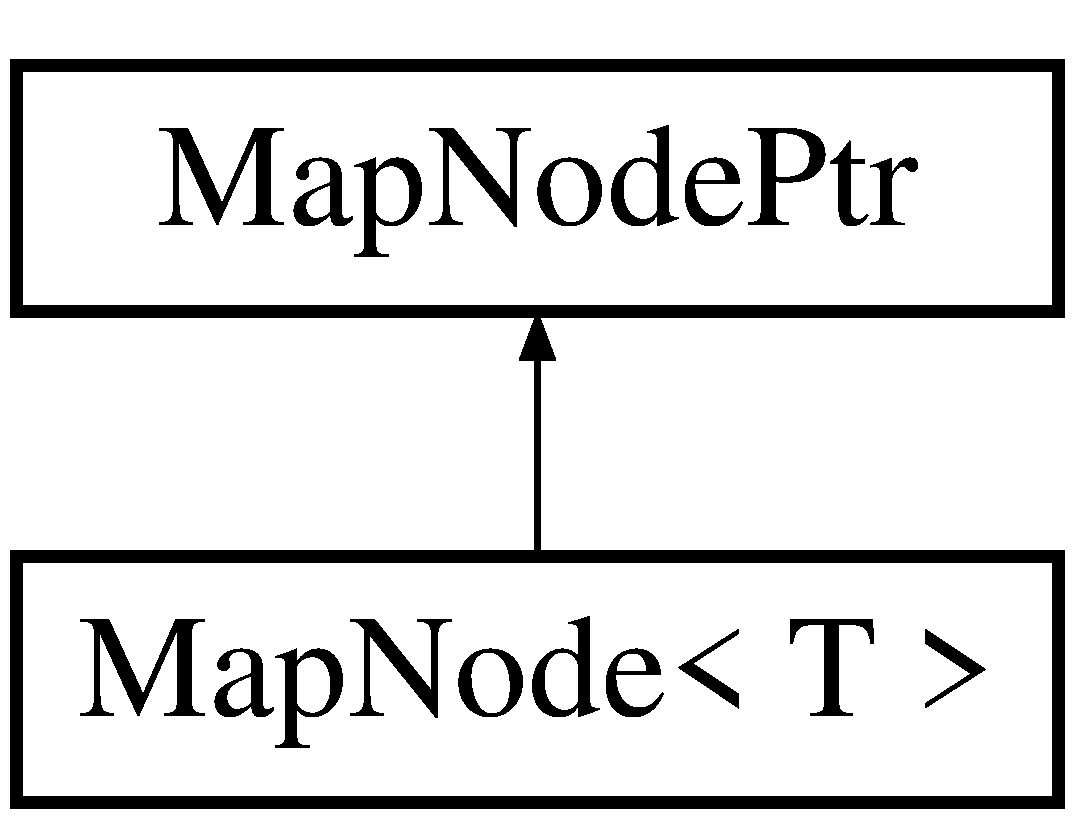
\includegraphics[height=2.000000cm]{classMapNode}
\end{center}
\end{figure}
\subsection*{Public Member Functions}
\begin{DoxyCompactItemize}
\item 
T $\ast$ \hyperlink{classMapNode_aac2d9cb3f7ae4f2e39a4ceaff588318c}{get\+Data} ()
\item 
char $\ast$ \hyperlink{classMapNode_aec1d6c32ce5cf507bdf8459cdd9a00b8}{get\+Data\+String} ()
\item 
void \hyperlink{classMapNode_a78cc24f37a1d1b4bda5075284ff53f92}{set\+Data} (char $\ast$data\+\_\+array)
\item 
\hyperlink{classMapNode_aa1dc56c3ee0462fd30f11f70a758002d}{Map\+Node} (std\+::string n, T $\ast$d)
\item 
\hyperlink{classMapNode_a56f35b20fd5e5bcc8425640f95512fd9}{Map\+Node} (std\+::string n, T $\ast$d, size\+\_\+t d\+L)
\end{DoxyCompactItemize}
\subsection*{Protected Attributes}
\begin{DoxyCompactItemize}
\item 
T $\ast$ \hyperlink{classMapNode_a61524bb1f8518fb99166e8880b065c9e}{data}
\end{DoxyCompactItemize}
\subsection*{Additional Inherited Members}


\subsection{Detailed Description}
\subsubsection*{template$<$typename T$>$class Map\+Node$<$ T $>$}

\hyperlink{classMapNode}{Map\+Node} Class  Template that catalogues and serializes an object of any type as well as take in a raw char$\ast$ representation of that data and parse it back into the correct format \begin{DoxyAttention}{Attention}
only works with P\+O\+D types without padded data (i.\+e no structs, unions) if an object is not guaranteed to have contiguous data, Y\+O\+U M\+U\+S\+T specialize the template in order to use it 
\end{DoxyAttention}


\subsection{Constructor \& Destructor Documentation}
\hypertarget{classMapNode_aa1dc56c3ee0462fd30f11f70a758002d}{\index{Map\+Node@{Map\+Node}!Map\+Node@{Map\+Node}}
\index{Map\+Node@{Map\+Node}!Map\+Node@{Map\+Node}}
\subsubsection[{Map\+Node}]{\setlength{\rightskip}{0pt plus 5cm}template$<$typename T$>$ {\bf Map\+Node}$<$ T $>$\+::{\bf Map\+Node} (
\begin{DoxyParamCaption}
\item[{std\+::string}]{n, }
\item[{T $\ast$}]{d}
\end{DoxyParamCaption}
)\hspace{0.3cm}{\ttfamily [inline]}}}\label{classMapNode_aa1dc56c3ee0462fd30f11f70a758002d}
\hyperlink{classMapNode}{Map\+Node(string,\+T$\ast$)} with implicit data length \begin{DoxyItemize}
\item {\ttfamily n} \+: name of node \item {\ttfamily d} \+: pointer to the node data \begin{DoxyReturn}{Returns}
{\ttfamily void} 
\end{DoxyReturn}
\begin{DoxyAttention}{Attention}
only use if you are sure that sizeof(datatype) will give an accurate size 
\end{DoxyAttention}
\end{DoxyItemize}
\hypertarget{classMapNode_a56f35b20fd5e5bcc8425640f95512fd9}{\index{Map\+Node@{Map\+Node}!Map\+Node@{Map\+Node}}
\index{Map\+Node@{Map\+Node}!Map\+Node@{Map\+Node}}
\subsubsection[{Map\+Node}]{\setlength{\rightskip}{0pt plus 5cm}template$<$typename T$>$ {\bf Map\+Node}$<$ T $>$\+::{\bf Map\+Node} (
\begin{DoxyParamCaption}
\item[{std\+::string}]{n, }
\item[{T $\ast$}]{d, }
\item[{size\+\_\+t}]{d\+L}
\end{DoxyParamCaption}
)\hspace{0.3cm}{\ttfamily [inline]}}}\label{classMapNode_a56f35b20fd5e5bcc8425640f95512fd9}
\hyperlink{classMapNode}{Map\+Node(string,\+T$\ast$,size\+\_\+t)} with explicit data length \begin{DoxyItemize}
\item {\ttfamily n} \+: name of node \item {\ttfamily d} \+: pointer to the node data \item {\ttfamily d\+L} \+: length of array needed to hold serialized data \begin{DoxyReturn}{Returns}
{\ttfamily void} 
\end{DoxyReturn}
\begin{DoxyAttention}{Attention}
data length is N\+O\+T N\+E\+C\+E\+S\+S\+A\+R\+I\+L\+Y the size of the object, it is the length of the array needed to hold the serialized data 
\end{DoxyAttention}
\end{DoxyItemize}


\subsection{Member Function Documentation}
\hypertarget{classMapNode_aac2d9cb3f7ae4f2e39a4ceaff588318c}{\index{Map\+Node@{Map\+Node}!get\+Data@{get\+Data}}
\index{get\+Data@{get\+Data}!Map\+Node@{Map\+Node}}
\subsubsection[{get\+Data}]{\setlength{\rightskip}{0pt plus 5cm}template$<$typename T$>$ T$\ast$ {\bf Map\+Node}$<$ T $>$\+::get\+Data (
\begin{DoxyParamCaption}
{}
\end{DoxyParamCaption}
)\hspace{0.3cm}{\ttfamily [inline]}}}\label{classMapNode_aac2d9cb3f7ae4f2e39a4ceaff588318c}
\hyperlink{classMapNode_aac2d9cb3f7ae4f2e39a4ceaff588318c}{get\+Data()} \begin{DoxyItemize}
\item {\ttfamily void} \begin{DoxyReturn}{Returns}
{\ttfamily \&data} \+: a pointer to the node data 
\end{DoxyReturn}
\end{DoxyItemize}
\hypertarget{classMapNode_aec1d6c32ce5cf507bdf8459cdd9a00b8}{\index{Map\+Node@{Map\+Node}!get\+Data\+String@{get\+Data\+String}}
\index{get\+Data\+String@{get\+Data\+String}!Map\+Node@{Map\+Node}}
\subsubsection[{get\+Data\+String}]{\setlength{\rightskip}{0pt plus 5cm}template$<$typename T$>$ char$\ast$ {\bf Map\+Node}$<$ T $>$\+::get\+Data\+String (
\begin{DoxyParamCaption}
{}
\end{DoxyParamCaption}
)\hspace{0.3cm}{\ttfamily [inline]}, {\ttfamily [virtual]}}}\label{classMapNode_aec1d6c32ce5cf507bdf8459cdd9a00b8}
\hyperlink{classMapNode_aec1d6c32ce5cf507bdf8459cdd9a00b8}{get\+Data\+String()} \begin{DoxyItemize}
\item {\ttfamily void} \begin{DoxyReturn}{Returns}
{\ttfamily data\+\_\+array} \+: a raw char$\ast$ array of the data 
\end{DoxyReturn}
\begin{DoxyAttention}{Attention}
One of the two methods (\hyperlink{classMapNode_aec1d6c32ce5cf507bdf8459cdd9a00b8}{get\+Data\+String()} and \hyperlink{classMapNode_a78cc24f37a1d1b4bda5075284ff53f92}{set\+Data(char $\ast$)} ) that need to be specialized if using custom types 
\end{DoxyAttention}
\end{DoxyItemize}


Implements \hyperlink{classMapNodePtr_a2d7366a2f34c69877a05e8afbaa92d01}{Map\+Node\+Ptr}.

\hypertarget{classMapNode_a78cc24f37a1d1b4bda5075284ff53f92}{\index{Map\+Node@{Map\+Node}!set\+Data@{set\+Data}}
\index{set\+Data@{set\+Data}!Map\+Node@{Map\+Node}}
\subsubsection[{set\+Data}]{\setlength{\rightskip}{0pt plus 5cm}template$<$typename T$>$ void {\bf Map\+Node}$<$ T $>$\+::set\+Data (
\begin{DoxyParamCaption}
\item[{char $\ast$}]{data\+\_\+array}
\end{DoxyParamCaption}
)\hspace{0.3cm}{\ttfamily [inline]}, {\ttfamily [virtual]}}}\label{classMapNode_a78cc24f37a1d1b4bda5075284ff53f92}
\hyperlink{classMapNode_a78cc24f37a1d1b4bda5075284ff53f92}{set\+Data(char$\ast$)} \begin{DoxyItemize}
\item {\ttfamily data\+\_\+array} \+: a raw char$\ast$ array of the data \begin{DoxyReturn}{Returns}
{\ttfamily void} 
\end{DoxyReturn}
\begin{DoxyAttention}{Attention}
One of the two methods (\hyperlink{classMapNode_aec1d6c32ce5cf507bdf8459cdd9a00b8}{get\+Data\+String()} and \hyperlink{classMapNode_a78cc24f37a1d1b4bda5075284ff53f92}{set\+Data(char $\ast$)} ) that need to be specialized if using custom types 
\end{DoxyAttention}
\end{DoxyItemize}


Implements \hyperlink{classMapNodePtr_aefd9101ca6bee00cd3304e72b2ca50bb}{Map\+Node\+Ptr}.



\subsection{Member Data Documentation}
\hypertarget{classMapNode_a61524bb1f8518fb99166e8880b065c9e}{\index{Map\+Node@{Map\+Node}!data@{data}}
\index{data@{data}!Map\+Node@{Map\+Node}}
\subsubsection[{data}]{\setlength{\rightskip}{0pt plus 5cm}template$<$typename T$>$ T$\ast$ {\bf Map\+Node}$<$ T $>$\+::data\hspace{0.3cm}{\ttfamily [protected]}}}\label{classMapNode_a61524bb1f8518fb99166e8880b065c9e}
pointer to data 

The documentation for this class was generated from the following file\+:\begin{DoxyCompactItemize}
\item 
D\+G\+R\+\_\+framework.\+h\end{DoxyCompactItemize}

\hypertarget{classMapNodePtr}{\section{Map\+Node\+Ptr Class Reference}
\label{classMapNodePtr}\index{Map\+Node\+Ptr@{Map\+Node\+Ptr}}
}


{\ttfamily \#include $<$D\+G\+R\+\_\+framework.\+h$>$}

Inheritance diagram for Map\+Node\+Ptr\+:\begin{figure}[H]
\begin{center}
\leavevmode
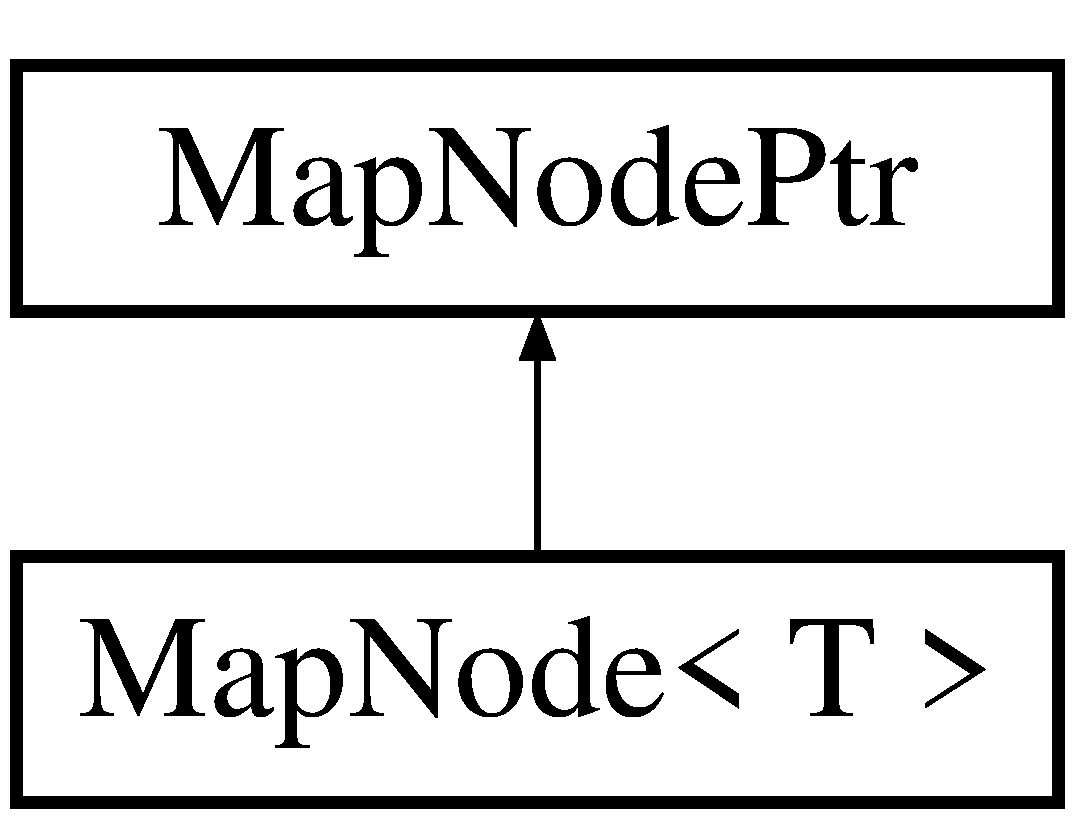
\includegraphics[height=2.000000cm]{classMapNodePtr}
\end{center}
\end{figure}
\subsection*{Public Member Functions}
\begin{DoxyCompactItemize}
\item 
virtual char $\ast$ \hyperlink{classMapNodePtr_a2d7366a2f34c69877a05e8afbaa92d01}{get\+Data\+String} ()=0
\item 
virtual void \hyperlink{classMapNodePtr_aefd9101ca6bee00cd3304e72b2ca50bb}{set\+Data} (char $\ast$)=0
\item 
\hyperlink{classMapNodePtr_ace653557c82003ba13ad9aa663bdc25f}{Map\+Node\+Ptr} (std\+::string n)
\item 
\hypertarget{classMapNodePtr_ab5ed81d4fe235d9df10a66088ed1ef76}{{\bfseries Map\+Node\+Ptr} (std\+::string n, size\+\_\+t d\+L)}\label{classMapNodePtr_ab5ed81d4fe235d9df10a66088ed1ef76}

\end{DoxyCompactItemize}
\subsection*{Public Attributes}
\begin{DoxyCompactItemize}
\item 
std\+::string \hyperlink{classMapNodePtr_a928378e3e8b1661858463cedc8e721c9}{name}
\item 
size\+\_\+t \hyperlink{classMapNodePtr_ac90162a897b772218843f49b4b08dc06}{data\+Length}
\end{DoxyCompactItemize}


\subsection{Detailed Description}
\hyperlink{classMapNodePtr}{Map\+Node\+Ptr} Class  Class that allows for us to have a multi-\/type map. Anything that goes into the input map must extend this class \begin{DoxyAttention}{Attention}
contains virtual functions and is intended to be extended by other classes. Do not try to use without pointing to a \hyperlink{classMapNode}{Map\+Node} 
\end{DoxyAttention}


\subsection{Constructor \& Destructor Documentation}
\hypertarget{classMapNodePtr_ace653557c82003ba13ad9aa663bdc25f}{\index{Map\+Node\+Ptr@{Map\+Node\+Ptr}!Map\+Node\+Ptr@{Map\+Node\+Ptr}}
\index{Map\+Node\+Ptr@{Map\+Node\+Ptr}!Map\+Node\+Ptr@{Map\+Node\+Ptr}}
\subsubsection[{Map\+Node\+Ptr}]{\setlength{\rightskip}{0pt plus 5cm}Map\+Node\+Ptr\+::\+Map\+Node\+Ptr (
\begin{DoxyParamCaption}
\item[{std\+::string}]{n}
\end{DoxyParamCaption}
)\hspace{0.3cm}{\ttfamily [inline]}}}\label{classMapNodePtr_ace653557c82003ba13ad9aa663bdc25f}
\hyperlink{classMapNodePtr}{Map\+Node\+Ptr(string)} \begin{DoxyItemize}
\item {\ttfamily n} \+: name of node \begin{DoxyReturn}{Returns}
{\ttfamily void} 
\end{DoxyReturn}
\begin{DoxyAttention}{Attention}
only use if you assign data\+Length a value 
\end{DoxyAttention}
\end{DoxyItemize}


\subsection{Member Function Documentation}
\hypertarget{classMapNodePtr_a2d7366a2f34c69877a05e8afbaa92d01}{\index{Map\+Node\+Ptr@{Map\+Node\+Ptr}!get\+Data\+String@{get\+Data\+String}}
\index{get\+Data\+String@{get\+Data\+String}!Map\+Node\+Ptr@{Map\+Node\+Ptr}}
\subsubsection[{get\+Data\+String}]{\setlength{\rightskip}{0pt plus 5cm}virtual char$\ast$ Map\+Node\+Ptr\+::get\+Data\+String (
\begin{DoxyParamCaption}
{}
\end{DoxyParamCaption}
)\hspace{0.3cm}{\ttfamily [pure virtual]}}}\label{classMapNodePtr_a2d7366a2f34c69877a05e8afbaa92d01}
get\+Data\+String \begin{DoxyItemize}
\item {\ttfamily void} \begin{DoxyReturn}{Returns}
{\ttfamily data\+\_\+array} \+: a raw char$\ast$ array of the data 
\end{DoxyReturn}
\begin{DoxyAttention}{Attention}
virtual function! 
\end{DoxyAttention}
\end{DoxyItemize}


Implemented in \hyperlink{classMapNode_aec1d6c32ce5cf507bdf8459cdd9a00b8}{Map\+Node$<$ T $>$}.

\hypertarget{classMapNodePtr_aefd9101ca6bee00cd3304e72b2ca50bb}{\index{Map\+Node\+Ptr@{Map\+Node\+Ptr}!set\+Data@{set\+Data}}
\index{set\+Data@{set\+Data}!Map\+Node\+Ptr@{Map\+Node\+Ptr}}
\subsubsection[{set\+Data}]{\setlength{\rightskip}{0pt plus 5cm}virtual void Map\+Node\+Ptr\+::set\+Data (
\begin{DoxyParamCaption}
\item[{char $\ast$}]{}
\end{DoxyParamCaption}
)\hspace{0.3cm}{\ttfamily [pure virtual]}}}\label{classMapNodePtr_aefd9101ca6bee00cd3304e72b2ca50bb}
get\+Data\+String \begin{DoxyItemize}
\item {\ttfamily data\+\_\+array} \+: a raw char$\ast$ array of the data \begin{DoxyReturn}{Returns}
{\ttfamily void} 
\end{DoxyReturn}
\begin{DoxyAttention}{Attention}
virtual function! 
\end{DoxyAttention}
\end{DoxyItemize}


Implemented in \hyperlink{classMapNode_a78cc24f37a1d1b4bda5075284ff53f92}{Map\+Node$<$ T $>$}.



\subsection{Member Data Documentation}
\hypertarget{classMapNodePtr_ac90162a897b772218843f49b4b08dc06}{\index{Map\+Node\+Ptr@{Map\+Node\+Ptr}!data\+Length@{data\+Length}}
\index{data\+Length@{data\+Length}!Map\+Node\+Ptr@{Map\+Node\+Ptr}}
\subsubsection[{data\+Length}]{\setlength{\rightskip}{0pt plus 5cm}size\+\_\+t Map\+Node\+Ptr\+::data\+Length}}\label{classMapNodePtr_ac90162a897b772218843f49b4b08dc06}
length of array holding serialized data \hypertarget{classMapNodePtr_a928378e3e8b1661858463cedc8e721c9}{\index{Map\+Node\+Ptr@{Map\+Node\+Ptr}!name@{name}}
\index{name@{name}!Map\+Node\+Ptr@{Map\+Node\+Ptr}}
\subsubsection[{name}]{\setlength{\rightskip}{0pt plus 5cm}std\+::string Map\+Node\+Ptr\+::name}}\label{classMapNodePtr_a928378e3e8b1661858463cedc8e721c9}
name of data node 

The documentation for this class was generated from the following file\+:\begin{DoxyCompactItemize}
\item 
D\+G\+R\+\_\+framework.\+h\end{DoxyCompactItemize}

%--- End generated contents ---

% Index
\newpage
\phantomsection
\addcontentsline{toc}{chapter}{Index}
\printindex

\end{document}
